%!tex program = lualatex
\documentclass[answers]{exam}
\usepackage{ctex}
\usepackage{graphicx}
\usepackage[margin=2cm]{geometry}
\usepackage{amsmath}
\usepackage{csquotes}
\usepackage{amssymb}
\usepackage{tikz}
\usetikzlibrary{
backgrounds,
calc,
decorations.pathmorphing,
decorations.pathreplacing,
decorations.text,
intersections,
patterns,
shapes,
shapes.symbols,
}
\pagestyle{empty}
\newcounter{xcord}
\newcounter{ycord}
\newcounter{total}
% \ctexset{
% 	subsection/name = {第,题},
% 	subsection/number = {\thesubsection},
% 	section ={
% 		name = {第,部分}
% 	}
% }
\renewcommand{\labelenumi}{\textbf{\ifnum\value{enumi}<10 0\fi\arabic{enumi})}}

\includeonly{svsu2022}
\begin{document}
%!tex program = lualatex
\documentclass{exam}
\usepackage{ctex}
\usepackage{graphicx}
\usepackage[margin=2cm]{geometry}
\usepackage{amsmath, amssymb}
\usepackage{csquotes}
\usepackage{tikz, pgfplots}
\usetikzlibrary{
	angles,
	backgrounds,
	calc,
	decorations.pathmorphing,
	decorations.pathreplacing,
	decorations.text,
	intersections,
	patterns,
	quotes,
	shapes,
	shapes.symbols,
}
\pagestyle{empty}
\newcounter{xcord}
\newcounter{ycord}
\newcounter{total}
\renewcommand{\labelenumi}{\textbf{\ifnum\value{enumi}<10 0\fi\arabic{enumi})}}

\pgfplotsset{compat=1.18}

\CorrectChoiceEmphasis{\color{blue!70!green}\bfseries}
\renewcommand{\solutiontitle}{\textbf{解:}}

\usepackage{array, tabularx}
\newcolumntype{C}{>{\centering\arraybackslash}X}
\newcolumntype{B}{>{\centering\bfseries\arraybackslash}X}
\catcode`\幺=0

\begin{document}
\section{求阴影面积}
\begin{figure}[htbp]
	\centering
	\begin{gather*}
		长方形ABCD\\
		AB = 9 \\
		BC = 6 \\
		求阴影面积
	\end{gather*}
	\begin{tikzpicture}[scale=.5]
		\coordinate (A) at (9,0);
		\coordinate (B) at (0,0);
		\coordinate (C) at (0,-6);
		\coordinate (D) at (9, -6);
		\coordinate (E) at (3, 0);
		\coordinate (F) at (5, -6);
		\coordinate (C') at (9, -3);
		\coordinate (B') at ($(C') ! 1.2 ! -90:(F)$);
		\path [name path=B'C'] (B') -- (C');
		\path [name path=AE] (A) -- (E);

		\draw [name intersections={of=B'C' and AE, by=G}];
		\node [above right] at(G){$G$};

		% \path[draw=red] {AE};

		\draw[dashed](B) -- (E);
		\draw (E)-- (A) -- (D) -- (F) -- (E);
		\draw[dashed] (F) -- (C) -- (B);
		\draw (F) -- (C') -- (B') -- (E);

		\draw [pattern=north east lines](E) -- (G) -- (C') -- (F) -- cycle;
		\node at (A)[above right]{$A$};
		\node at (B)[above left]{$B$};
		\node at (C)[below left]{$C$};
		\node at (D)[below right]{$D$};
		\node at (F)[below]{$F$};
		\node at (C')[right]{$C\prime$ 中点};
		\node at (E)[above left]{$E$};
		\node at (B')[right, xshift=5pt]{$B\prime$};
	\end{tikzpicture}
\end{figure}

\begin{align}
	FC + FD                    & = 9                      \\
	FC^2                       & = FD^2 + DC^2 = FD^2 + 9 \\
	(FC + FD) \times (FC - FD) & = 9                      \\
	FC - FD                    & = 1                      \\
	FC                         & = 5
\end{align}

Calculate the length of $BE$:
\begin{align}
	\triangle CDF            & \approx \triangle CAG                               \\
	\frac{GA}{AC}            & = \frac{CD}{FD} = \frac{3}{4}                       \\
	GA                       & = \frac{9}{4}                                       \\
	GC                       & = \sqrt{GA^2 + AC^2} = \frac{15}{4}                 \\
	BG                       & = BC - GC = 6 - \frac{15}{4}     = \frac{9}{4} = GA \\
	\because \triangle GBE   & \approx \triangle GAC                               \\
	\therefore \triangle GBE & \cong \triangle GAC                                 \\
	BE                       & = AC = 3
\end{align}

\section*{20以内两位数乘法练习}
\begin{center}
	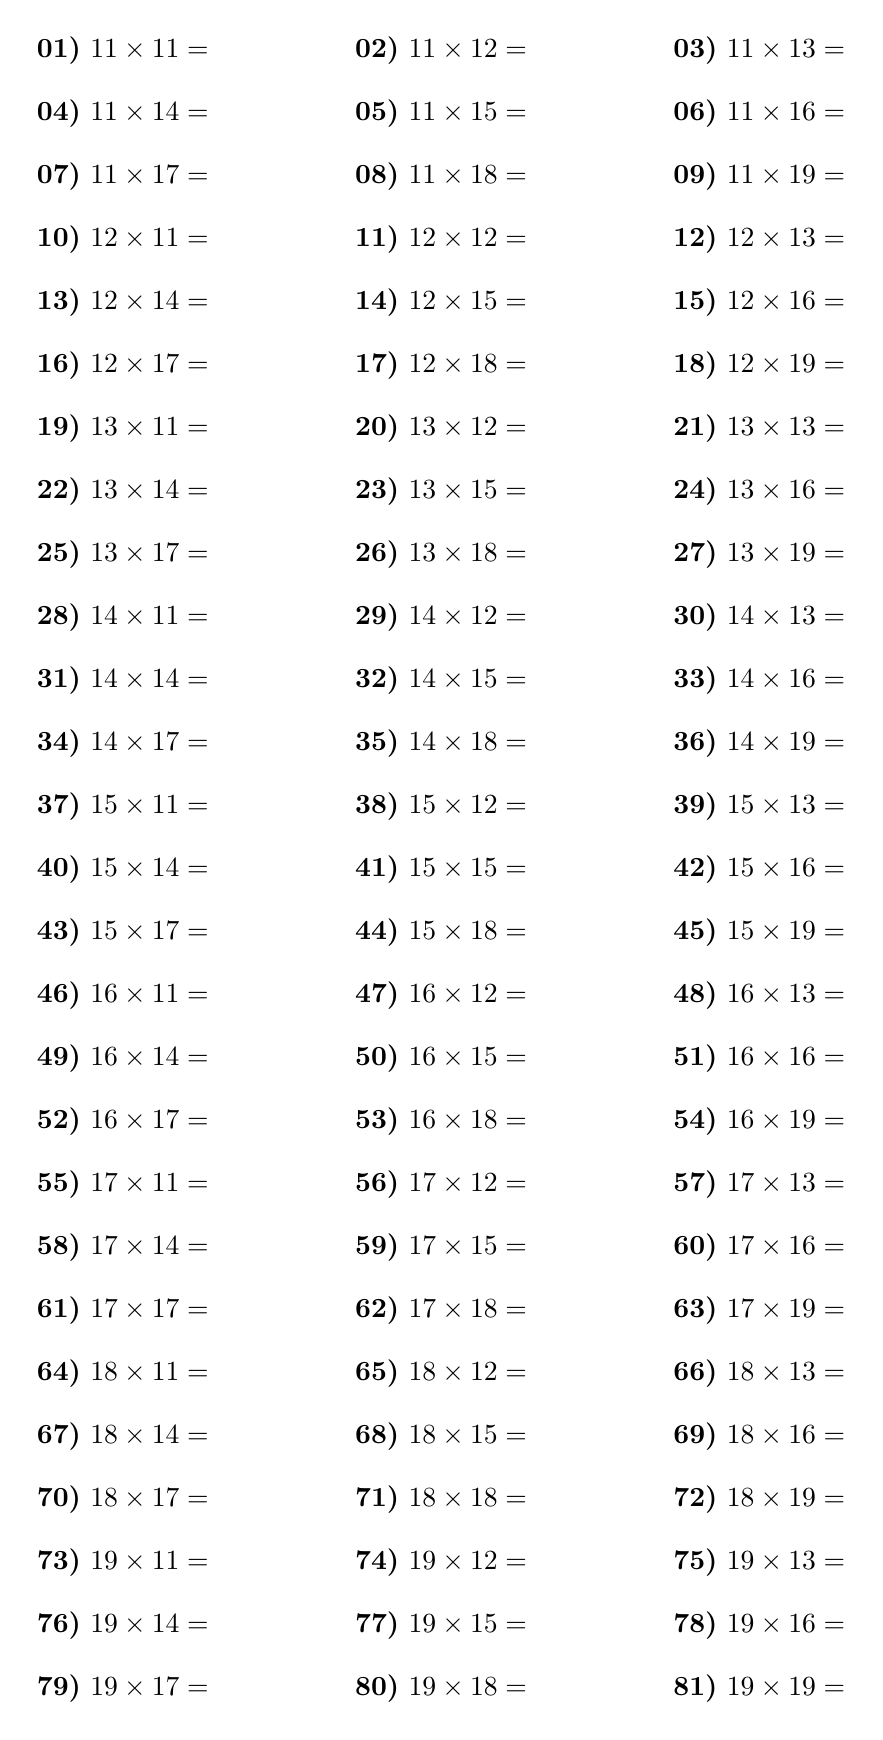
\begin{tikzpicture}
		\foreach \x in {11,...,19}
		\foreach \y in {11,...,19}
			{
				\stepcounter{total}
				\node at (\value{xcord} * \textwidth / 3, -\value{ycord}*0.8) {\textbf{\ifnum\value{total}<10
				0\fi\thetotal)} $\x \times \y =$};
		\stepcounter{xcord}		\ifnum\value{xcord}=3
		\setcounter{xcord}{0}
		\stepcounter{ycord}
		\fi
		}
	\end{tikzpicture}

\end{center}

\section{速算及巧算}
\subsection{计算总和}
\begin{enumerate}
	\item $1-2+3-4+5-6+7-8+9-10+11=$

	\item $3+5+7+9+11+13+15+17+19+21=$

	\item $100-99+98-97+96-95+94-93+93-92+91=$

	\item $6+8+10+12+14+16+18+20+22+24=$

	\item $1 + 2 + 3 + \ldots + 100 = $

	\item $2 + 4 +6 + \ldots + 100 = $

	\item $1 + 3 + 5 + \ldots + 99 = $

	\item $5 + 10 + 15 + \ldots + 100 = $

	\item $1 - (1+2) + (1+2+3) - (1+2+3+4) + \ldots - (1+2+\ldots+98) + (1+2+\ldots+99) = $

	\item $1-2+3-4+\ldots+2023-2024+2025=$

	\item $19+28+37+46+55+64+73+82+91+ \underline{\hspace{1cm}}=550$

	\item $2000-180+220-180+220-180+220-180+220-180+220=$

	\item $352.46-35.58-65.93-76.07-24.42=$

	\item $1+2+4+8+16+32+64+128+256+512+1024=$

	\item $8+89+899+8999+89999=$

	\item $8+88+888+8888+88888=$

	\item $28+208+2008+20008=$

	\item $24+63+52+17+49+81+74+38+95=$

	\item $1999.9+199.9+19.9+1.9=$

	\item $(7+9+11+13+\ldots+37)-(9+11+13+15+\ldots+35)=$

\end{enumerate}

\pagebreak
\section{速算和巧算2}

\begin{enumerate}

	\item $(6+8+10+12+\ldots+36)-(8+10+12+14+\ldots+34)=$

	\item $(1+4+7+10+\ldots+40)-(4+7+10+13+\ldots+37)=$
\end{enumerate}
\end{document}

\section{SVSU2022 level1}
\begin{questions}
	\question 考虑方程$p(x): ax^2 + bx + c=0$,其系数$a$,$b$和$c$都是非零的,并且每个系数都满足从方程$p(x)$
	中移除包含该系数的项后得到的方程;例如,系数$b$是方程 $ax^2+c=0$的一个解。求方程$p(x)$
	所有解的和是多少?

	\begin{oneparchoices}
		\CorrectChoice 总是 1 \choice 总是 -1 \choice 总是 2 \choice 1 或者 -1 \choice 1 或者 2
	\end{oneparchoices}
	\begin{solution}
		方程$p(x)$的两个解分别为$\displaystyle x_1, x_2 = \frac{-b \pm \sqrt{b^2 - 4ac}}{2a}$,则$\displaystyle x_1 +
			x_2 = -\frac{b}{a}$\\
		由题意得
		\begin{align}
			ac^2  + bc & = 0 \label{\thequestion:1} \\
			ab^2  + c  & = 0 \label{\thequestion:2} \\
			ab    + c  & = 0 \label{\thequestion:3}
		\end{align}
		由式(\ref{\thequestion:2}) 和(\ref{\thequestion:3})得$b=1$和$a+c=0$,代入(\ref{\thequestion:1})得:
		\begin{equation}
			a(-a) -a  = 0
		\end{equation}

		则$a=-1$或$a=0$,因为题目中$a \ne 0$,所以$a=-1$,则$\displaystyle x_1 + x_2 = -\frac{b}{a}=1$
	\end{solution}
	\question 一支行进乐队共有150名成员。有一天,只有部分成员到场,但没有人想花时间去清点具体人数。他们首先尝试以每排5名成员的方式排队,但结果多出了1名成员。接着他们改以每排6名成员的方式排列,仍然多出了1名成员。最后,他们尝试以每排7名成员的方式排列,这次多出了2名成员。请问,为了确保没有成员被剩下,他们应该以每排多少人的方式排列?

	\begin{oneparchoices}
		\choice 4人每排
		\CorrectChoice 11人每排
		\choice 13人每排
		\choice 17人每排
		\choice 上述选项中无正确答案
	\end{oneparchoices}
	\begin{solution}
		设当天一共到场$x$人, 根据题意得
		\begin{equation}
			\begin{cases}
				x \equiv 1 \pmod 5 \\
				x \equiv 1 \pmod 6
			\end{cases}
		\end{equation}
		则$x=k(5 \times 6) + 1$,其中$k=0,1,2,3 \ldots$

		根据总人数小于150这个条件,$x$可能的值有$1,31,61,91,121$,然后根据每排排7人的情况下多出2名成员,得到$x=121$,则每排11个人可以确保没有成员被剩下。

	\end{solution}

	\question 下列陈述中,哪一个是唯一正确的?
	\begin{choices}
		\choice 水平线的图形不可能有任何与x轴的交点。
		\CorrectChoice 水平线的图形不能有一个唯一的与x轴的交点,但可能有超过一个与x轴的交点。
		\choice 抛物线的图形不能有一个唯一的与x轴的交点,但可能有超过一个与x轴的交点。
		\choice 三次或更高次的多项式的图形必须至少有一个与x轴的交点。
		\choice 要么没有一个是正确的,要么不止一个正确。
	\end{choices}
	\begin{solution}\\
		选项A:当$x=0$时与$x$轴有无穷多个交点。\\
		选项B:根据以上,此描述正确。\\
		选项C:当抛物线的顶点位于$x$轴上时有唯一的交点,所以此描述错误。\\
		选项D:比如$x^4+1$这样的曲线就没有与$x$轴的交点,所以此描述错误。
	\end{solution}

	\question 下列哪个选项等于10的阶乘($10!$)。如果你对符号不熟悉,$n!$(读作\enquote{n的阶乘})对于任何非负整数$n$定义如下:
	\begin{equation*}
		\begin{cases}
			0! = 1 \\
			n > 0,n! = n \cdot (n-1)!
		\end{cases}
	\end{equation*}
	你需要从下面的选项中选择:

	\begin{oneparchoices}
		\choice $5! \cdot 2!$
		\CorrectChoice $7! \cdot 5! \cdot 3!$
		\choice $7! \cdot 5! \cdot 2!$
		\choice $7! \cdot 5! \cdot 3! \cdot 2!$ \\
		\choice 上述选项中没有符合条件的,或者有超过一个选项符合条件。
	\end{oneparchoices}

	\begin{solution}
		\begin{align*}
			10! & = 7! \cdot 8 \cdot 9 \cdot 10                        \\
			    & = 7! \cdot 2 \cdot 4 \cdot 3 \cdot 3 \cdot 2 \cdot 5 \\
			    & = 7! \cdot 5! \cdot 3!
		\end{align*}
	\end{solution}

	\question 一个数的六进制表示为550,另一个数的五进制表示为3440,求它们的最大公约数用4进制表示为多少。

	\begin{oneparchoices}
		\choice 24 \CorrectChoice 33 \choice 113 \choice 223 \choice 以上都不对
	\end{oneparchoices}

	\begin{solution}
		\begin{align*}
			550_{(6)}                    & = 5 \times 6^2 + 5 \times 6^1 + 0 \times 6^0                \\
			                             & = 210_{(10)}                                                \\
			3440_{(5)}                   & = 3 \times 5^3 + 4 \times 5^2 + 4 \times 5^1 + 0 \times 5^0 \\
			                             & = 495_{(10)}                                                \\
			\gcd(210_{(10)}, 495_{(10)}) & = 15_{(10)}                                                 \\
			                             & = 3 \times 4^1 + 3 \times 4^0                               \\
			                             & = 33_{(4)}
		\end{align*}

	\end{solution}

	\question
	一个人沿着海滩走,从点A开始,以每小时3公里的速度行走,并且在B点进入水中,以每小时2公里的速度斜向游到一个距离C点$\sqrt{3}$公里远的小岛上,直接横跨岛屿与海岸线相对的位置,如图所示。从A点到C点的总距离为3公里。有两种不同的选择,从A点到B点的距离(以公里为单位)将导致步行和游泳的总时间为一小时四十分钟;这两个数字之和是多少?

	\begin{oneparchoices}
		\choice 2 \choice 4 \CorrectChoice $\frac{14}{5}$ \choice $\frac{16}{5}$ \choice 以上都不对
	\end{oneparchoices}

	\begin{figure}[ht]
		\centering
		\begin{tikzpicture}[scale=0.8, every node/.style={transform shape}]
			% Define coordinates
			\coordinate (A) at (0,0);
			\coordinate (B) at (2,0);
			\coordinate (C) at (3,0);
			\coordinate (D) at (3,{sqrt(3)});

			% Draw horizontal lines for the sea
			\begin{scope}[on background layer]
				\draw[dashed] (A) -- (B);
				\draw[dashed] (B) -- (C);
				\draw[dashed] (C) -- (D);
				\draw[dashed] (B) -- (D);
			\end{scope}

			\node[fill=white] at (A){$A$};
			\node[fill=white] at (B){$B$};
			\node[fill=white] at (C){$C$};
			\node[cloud, draw=black, minimum width=3cm, minimum height=2cm, anchor=south] at (D){小岛};

			\draw[decoration={coil, segment length = 5mm, amplitude = 0.5mm}, decorate] ([yshift=0.5cm]A) -- ([yshift=0.5cm]C);
			\draw[decoration={brace, mirror}, decorate] ([yshift=-0.5cm]A) -- ([yshift=-0.5cm]C);
			\draw[decoration={brace, mirror}, decorate] ([xshift=0.5cm]C) -- ([xshift=0.5cm]D);
			\node at ([yshift=-1cm]$(A)!0.5!(C)$) {3公里};
			\node at ([xshift=1.5cm]$(C)!0.5!(D)$) {$\sqrt{3}$公里};

			\node at (0,2) {\~{}};
			\node at (1,1.5) {\~{}};
			\node at (2,1) {\~{}};
			\node at (2,1.5) {\~{}};

		\end{tikzpicture}
		\caption{\thequestion}
	\end{figure}

	\begin{solution}
		\begin{enumerate}
			\item 设$AB=x$,则$BC=3-x$
			\item 设$B$点到小岛的距离为$y$,则有
			      \begin{equation}
				      y^2 = (3-x)^2 + 3 \label{\thequestion:step2}
			      \end{equation}
			\item 根据总时间可以得
			      \begin{gather}
				      \frac{x}{3} + \frac{y}{2} = \frac{100}{60} = \frac{5}{3}\\
				      2x + 3y = 10 \\
				      y = \frac{10 - 2x}{3}
			      \end{gather}
			\item 将$y$代入式(\ref{\thequestion:step2})中,得
			      \begin{gather}
				      \frac{(10-2x)^2}{3^2} = 9 - 6x + x^2 + 3 \\
				      100 -40x + 4x^2 = 108 - 54x + 9x^2 \\
				      5x^2 -14x + 8 = 0 \label{\thequestion:step4}
			      \end{gather}
			\item 方程(\ref{\thequestion:step4})的两个解的和
			      \begin{equation}
				      x_1 + x_2 = \frac{-(-14) \times 2}{5 \times 2} = \frac{14}{5}
			      \end{equation}
		\end{enumerate}
	\end{solution}

	\question 下列哪个值与$|\sqrt{2022} - 45|$相等

	\begin{oneparchoices}
		\choice $\sqrt{3}$ \choice $\sqrt{1997}$ \choice $\sqrt{2022} - 45$ \choice $\sqrt{2022} + 45$ \CorrectChoice $45 - \sqrt{2022}$
	\end{oneparchoices}

	\begin{solution}
		\begin{gather*}
			\because 45 = \sqrt{2025} > \sqrt{2022} \\
			\therefore \sqrt{2022} - 45 < 0
		\end{gather*}
	\end{solution}

	\question $s$为非负数,下列哪个与$\sqrt[6]{s^5}\sqrt[9]{s}$相等

	\begin{oneparchoices}
		\choice $\sqrt[3]{s}$ \choice $\sqrt[2]{s^2}$ \choice $\sqrt[54]{s^5}$ \CorrectChoice $\sqrt[18]{s^{17}}$ \choice 以上都不对
	\end{oneparchoices}

	\begin{solution}
		\begin{align*}
			\sqrt[6]{s^5}\sqrt[9]{s} & = s^{\frac{5}{6}}s^{\frac{1}{9}} \\
			                         & = s^{\frac{5}{6} + \frac{1}{9}}  \\
			                         & = s^{\frac{51}{54}}              \\
			                         & = s^{\frac{17}{18}}              \\
			                         & = \sqrt[17]{s^{18}}
		\end{align*}
	\end{solution}

	\question \( 7^3 \)个小正方体堆叠成一个 \( 7 \times 7 \times 7 \)的大正方体,请问大正方体的表面有多少个小正方体?

	\begin{oneparchoices}
		\choice 127 \choice 134 \CorrectChoice 218 \choice 294 \choice 327
	\end{oneparchoices}

	\begin{solution}
		\begin{enumerate}
			\item 角点有8个
			\item 棱柱有12条,每条上有5个,共计60个
			\item 一共6个面,每个面中间有25个,共计150个
			\item 共计218个
		\end{enumerate}
	\end{solution}

	\question
	\begin{minipage}{0.7\textwidth}
		右边所展示的立方体的每一面都标有一个正整数,使得每一对相对面的数字的乘积都是相同的。找出所有面上数字之和的最低可能值。
	\end{minipage}
	\begin{minipage}{0.25\textwidth}
		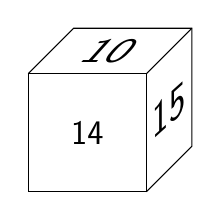
\begin{tikzpicture}[scale=0.5, every node/.style={scale=0.5}, baseline=(B)]
			\coordinate(A) at (0,0,0);
			\coordinate(B) at (0,3,0);
			\coordinate(C) at (3,3,0);
			\coordinate(D) at (3,0,0);
			\coordinate(E) at (0,0,3);
			\coordinate(F) at (0,3,3);
			\coordinate(G) at (3,3,3);
			\coordinate(H) at (3,0,3);

			\draw (E) -- (F) -- (G) -- (H) -- cycle;
			\draw (F) -- (B) -- (C) -- (D) -- (H);
			\draw (C) -- (G);

			\node at ($(E)!0.5!(G)$){\fontsize{64}{32}\selectfont\sf 14};
			\node[text effects={xslant=0.9}, xscale=1.4] at ($(F)!0.5!(C)$){\fontsize{40}{32}\selectfont\sf 10};
			\node [text effects={yslant=0.9}, yscale=1.4] at ($(H)!0.5!(C)$){\fontsize{36}{32}\selectfont\sf 15};
		\end{tikzpicture}
	\end{minipage}

	\begin{oneparchoices}
		\choice 78 \choice 80 \CorrectChoice 89 \choice 107 \choice 以上都不对
	\end{oneparchoices}
	\pagebreak
	\begin{solution}\\
		10、14、15三个数的最小公倍数为:210,则有
		\begin{equation*}
			\begin{cases}
				10\text{的对面是} 21 \\
				14\text{的对面是} 15 \\
				15\text{的对面是} 14
			\end{cases}
		\end{equation*}
	\end{solution}

	\question 找出下列比 \( \displaystyle \sqrt{22 + \sqrt{22 + \sqrt{22 + \sqrt{22}}}} \)小的最大整数。
	\begin{oneparchoices}
		\choice 4 \CorrectChoice 5 \choice 9 \choice 20 \choice 25
	\end{oneparchoices}
	\begin{solution}
		\begin{align*}
			\sqrt{22 + \sqrt{22 + \sqrt{22 + \sqrt{22}}}} & > \sqrt{22 + \sqrt{22 + \sqrt{22 + 4}}} \\
			                                              & > \sqrt{22 + \sqrt{22 + 5}}             \\
			                                              & > \sqrt{22 + 5}                         \\
			                                              & > 5
		\end{align*}
	\end{solution}

	\question 小明和小红正在用他们的计算器计算两个数 \( a \)和 \( b \)的平均值。首先,小明 使用计算器输入了 \( a + b
	\div 2 \) ,结果得到 \( 30 \)。然后小红使用相同的计算器输入了 \( b + a \div 2 \)结果得到 18。请问两个数的正确平均值是多少?

	\begin{oneparchoices}
		\choice 28 \choice 24 \CorrectChoice 16 \choice 12 \choice 以上都不对
	\end{oneparchoices}

	\begin{solution}
		\begin{align*}
			a    + b \div 2   & = 30 \\
			b    + a \div 2   & = 18 \\
			1.5  \times (a+b) & = 48 \\
			a    + b          & = 32 \\
		\end{align*}
		则正确的平均数为16。如果用常规的计算器是不会出现这种情况的。
	\end{solution}

	\question 下面的方程有几对整数解?
	\begin{equation}
		3x^2y - 10xy - 8y - 17 = 0
	\end{equation}
	\begin{oneparchoices}
		\choice 无 \CorrectChoice 1 \choice 2 \choice 4 \choice 以上都不对
	\end{oneparchoices}

	\begin{solution}
		\begin{align*}
			3x^2y - 10xy - 8y - 17 & = 0  \\
			y(3x^2 - 10x - 8)      & = 17 \\
			y(x-4)(3x+2)           & = 17 \\
		\end{align*}
		因为 \( 17 \) 是质数,所以只能有以下两种情况:
		\begin{equation*}
			\begin{cases}
				y = 1, \quad (x-4)(3x+2) = 17 \\
				y = 17,\quad  (x-4)(3x+2) = 1
			\end{cases}
		\end{equation*}
		在第一种情况下:
		\begin{align*}
			(x-4)(3x+2)     & = 17 \\
			3x^2 -10x - 25  & = 0  \\
			(3x + 5)(x - 5) & = 0  \\
		\end{align*}
		则 \( (x=5, y=1) \) 是方程的一组整数解。

		在第二种情况下:
		\begin{align*}
			3x^2 - 10x - 9 & = 0 \\
		\end{align*}
		此方程没有整数解。

		因此,题目中的方程只有一组整数解。
	\end{solution}

	\question  如果两只土拨鼠在12分钟内可以啃掉32斤的木头,那么三只土拨鼠在8分钟内可以啃掉多少斤的木头?
	\begin{oneparchoices}
		\choice \( 21\frac13 \) \CorrectChoice 32 \choice 64 \choice 80 \choice 以上都不对
	\end{oneparchoices}

	\begin{solution}
		\begin{align*}
			32 \div 12 \div 2 \times 3 \times 8 & = \frac{32 \times 3 \times 8}{12 \times 2} \\
			                                    & = 32
		\end{align*}
	\end{solution}

	\question 假设有打呼、磨牙、抽烟三种生活不良习惯,请问下列哪个系列的前提假设能够推断出老王不喝酒?

	\begin{oneparchoices}
	\choice 
	\begin{minipage}{0.25\textwidth}
	所有喝酒的人都磨牙\\ 
	磨牙的人不打呼 \\ 
	有些打呼的人抽烟 \\ 
	老王抽烟
	\end{minipage}
	\choice
	\begin{minipage}{0.25\textwidth}
		有些喝酒的人磨牙 \\
		没有磨牙的人会打呼 \\ 
		有些抽烟的人会打呼 \\ 
		老王抽烟
	\end{minipage}
	\choice
	\begin{minipage}{0.25\textwidth}
		所有喝酒的人磨牙 \\
		没有磨牙的人会打呼 \\ 
		所有打呼的人抽烟 \\ 
		老王抽烟
	\end{minipage}
	\CorrectChoice
	\begin{minipage}{0.25\textwidth}
		所有喝酒的人磨牙 \\
		没有磨牙的人会打呼 \\ 
		所有抽烟的人打呼 \\ 
		老王抽烟
	\end{minipage}
	\choice
	\begin{minipage}{0.25\textwidth}
		以上都不对
	\end{minipage}
	\end{oneparchoices}

	\begin{solution}

	A选项没有与喝酒相关的内容 \\ 
	B选项从老王抽烟与有些抽烟的人会打呼,只能推断出老王可能会打呼。
	从有些喝酒的人磨牙和没有磨牙的人会打呼,只能推断出有些喝酒的人不会打呼。\\ 
	C选项从老王抽烟,及所有打呼的人抽烟并不能推断出都比打呼 \\
	D选项从老王抽烟,以及所有抽烟的人打呼得出老王打呼\\ 
	从所有喝酒的人磨牙和没有磨牙的人会打呼得出喝酒的人不打呼,所以老王不喝酒


	\end{solution}

\end{questions}
\section{SVSU2022 level2}
\subsection{}
求
$\displaystyle\sum_{k=0}^{2022}\frac{2022!\cdot (-1)^k2^k}{k! \cdot (2022-k)!}$
的值

\subsection*{解:}
\begin{enumerate}
	\item 利用二项式定理$\displaystyle(x+y)^n = \sum_{k=0}^{n}\binom{n}{k}x^ky^{n-k}$
	      \begin{align}
		      \sum_{k=0}^{2022}\frac{2022!\cdot(-1)^k2^k}{k!\cdot(2022-k)!} & = \sum_{k=0}^{2022}\frac{2022!}{k!\cdot
		      (2022-k)!}(-2)^k                                                                                        \\
		                                                                    & =
		      \sum_{k=0}^{2022}\binom{2022}{k}(-2)^k\cdot 1^{2022-k}                                                  \\
		                                                                    & = (1-2)^{2022}                          \\
		                                                                    & = 1
	      \end{align}
\end{enumerate}

\subsection{}
求$(\sqrt[4]{27} + \sqrt{3} + \sqrt[4]{3} + 1)^2$
\subsection*{解:}
\begin{enumerate}
	\item 设$\displaystyle x=3^{\frac{1}{4}}$,则
	      \begin{align}
		      (\sqrt[4]{27} + \sqrt{3} + \sqrt[4]{3} + 1)^2 & = (x^3 + x^2 + x + 1)^2                     \\
		                                                    & = [x^2(x+1) + (x+1)]^2                      \\
		                                                    & = (x^2 + 1)^2(x+1)^2                        \\
		                                                    & = \frac{(x^2 + 1)^2(x+1)^2(x-1)^2}{(x-1)^2} \\
		                                                    & = \frac{(x^4 - 1)^2}{(x-1)^2}
	      \end{align}
	\item 将$x=\sqrt[4]{3}$代入得:
	      \begin{align}
		      \frac{(x^4 - 1)^2}{(x-1)^2} & = \frac{4}{(x-1)^2}                     \\
		                                  & = \frac{4}{x^2 - 2x + 1}                \\
		                                  & = \frac{4}{\sqrt{3} - 2\sqrt[4]{3} + 1}
	      \end{align}
\end{enumerate}

\end{document}
